\chapter{Cookbook -- Cool things to do with it}
\label{chapter:cookbook}

Biopython now has two collections of ``cookbook'' examples -- this chapter
(which has been included in this tutorial for many years and has gradually
grown), and \url{http://biopython.org/wiki/Category:Cookbook} which is a
user contributed collection on our wiki.

We're trying to encourage Biopython users to contribute their own examples
to the wiki. In addition to helping the community, one direct benefit of
sharing an example like this is that you could also get some feedback on
the code from other Biopython users and developers - which could help you
improve all your Python code.

In the long term, we may end up moving all of the examples in this chapter
to the wiki, or elsewhere within the tutorial.

\section{Working with sequence files}
\label{seq:cookbook-sequences}

This section shows some more examples of sequence input/output, using the
\verb|Bio.SeqIO| module described in Chapter~\ref{chapter:Bio.SeqIO}.

\subsection{Filtering a sequence file}

Often you'll have a large file with many sequences in it (e.g. FASTA file
or genes, or a FASTQ or SFF file of reads), a separate shorter list of
the IDs for a subset of sequences of interest, and want to make a new
sequence file for this subset.

Let's say the list of IDs is in a simple text file, as the first word on
each line. This could be a tabular file where the first column is the ID.
Try something like this:

%not a doctest to avoid temp files being left behind, also no >>>
%makes it easier to copy and paste the example to a script file.
\begin{verbatim}
from Bio import SeqIO
input_file = "big_file.sff"
id_file = "short_list.txt"
output_file = "short_list.sff"
wanted = set(line.rstrip("\n").split(None,1)[0] for line in open(id_file))
print("Found %i unique identifiers in %s" % (len(wanted), id_file))
records = (r for r in SeqIO.parse(input_file, "sff") if r.id in wanted)
count = SeqIO.write(records, output_file, "sff")
print("Saved %i records from %s to %s" % (count, input_file, output_file))
if count < len(wanted):
    print("Warning %i IDs not found in %s" % (len(wanted)-count, input_file))
\end{verbatim}

Note that we use a Python \verb|set| rather than a \verb|list|, this makes
testing membership faster.

\subsection{Producing randomised genomes}

Let's suppose you are looking at genome sequence, hunting for some sequence
feature -- maybe extreme local GC\% bias, or possible restriction digest sites.
Once you've got your Python code working on the real genome it may be sensible
to try running the same search on randomised versions of the same genome for
statistical analysis (after all, any ``features'' you've found could just be
there just by chance).

For this discussion, we'll use the GenBank file for the pPCP1 plasmid from
\textit{Yersinia pestis biovar Microtus}.  The file is included with the
Biopython unit tests under the GenBank folder, or you can get it from our
website, \href{http://biopython.org/SRC/biopython/Tests/GenBank/NC_005816.gb}
{\texttt{NC\_005816.gb}}.
This file contains one and only one record, so we can read it in as a
\verb|SeqRecord| using the \verb|Bio.SeqIO.read()| function:

%doctest ../Tests/GenBank
\begin{verbatim}
>>> from Bio import SeqIO
>>> original_rec = SeqIO.read("NC_005816.gb", "genbank")
\end{verbatim}

So, how can we generate a shuffled versions of the original sequence?  I would
use the built in Python \verb|random| module for this, in particular the function
\verb|random.shuffle| -- but this works on a Python list.  Our sequence is a
\verb|Seq| object, so in order to shuffle it we need to turn it into a list:

%cont-doctest
\begin{verbatim}
>>> import random
>>> nuc_list = list(original_rec.seq)
>>> random.shuffle(nuc_list) #acts in situ!
\end{verbatim}

Now, in order to use \verb|Bio.SeqIO| to output the shuffled sequence, we need
to construct a new \verb|SeqRecord| with a new \verb|Seq| object using this
shuffled list.  In order to do this, we need to turn the list of nucleotides
(single letter strings) into a long string -- the standard Python way to do
this is with the string object's join method.

%cont-doctest
\begin{verbatim}
>>> from Bio.Seq import Seq
>>> from Bio.SeqRecord import SeqRecord
>>> shuffled_rec = SeqRecord(Seq("".join(nuc_list), original_rec.seq.alphabet),
...                          id="Shuffled", description="Based on %s" % original_rec.id)
\end{verbatim}

Let's put all these pieces together to make a complete Python script which
generates a single FASTA file containing 30 randomly shuffled versions of
the original sequence.

This first version just uses a big for loop and writes out the records one by one
(using the \verb|SeqRecord|'s format method described in
Section~\ref{sec:Bio.SeqIO-and-StringIO}):

\begin{verbatim}
import random
from Bio.Seq import Seq
from Bio.SeqRecord import SeqRecord
from Bio import SeqIO

original_rec = SeqIO.read("NC_005816.gb","genbank")

handle = open("shuffled.fasta", "w")
for i in range(30):
    nuc_list = list(original_rec.seq)
    random.shuffle(nuc_list)
    shuffled_rec = SeqRecord(Seq("".join(nuc_list), original_rec.seq.alphabet), \
                             id="Shuffled%i" % (i+1), \
                             description="Based on %s" % original_rec.id)
    handle.write(shuffled_rec.format("fasta"))
handle.close()
\end{verbatim}

Personally I prefer the following version using a function to shuffle the record
and a generator expression instead of the for loop:

\begin{verbatim}
import random
from Bio.Seq import Seq
from Bio.SeqRecord import SeqRecord
from Bio import SeqIO

def make_shuffle_record(record, new_id):
    nuc_list = list(record.seq)
    random.shuffle(nuc_list)
    return SeqRecord(Seq("".join(nuc_list), record.seq.alphabet), \
           id=new_id, description="Based on %s" % original_rec.id)

original_rec = SeqIO.read("NC_005816.gb","genbank")
shuffled_recs = (make_shuffle_record(original_rec, "Shuffled%i" % (i+1)) \
                 for i in range(30))
handle = open("shuffled.fasta", "w")
SeqIO.write(shuffled_recs, handle, "fasta")
handle.close()
\end{verbatim}

\subsection{Translating a FASTA file of CDS entries}
\label{sec:SeqIO-translate}
Suppose you've got an input file of CDS entries for some organism, and you
want to generate a new FASTA file containing their protein sequences.  i.e.
Take each nucleotide sequence from the original file, and translate it.
Back in Section~\ref{sec:translation} we saw how to use the \verb|Seq|
object's \verb|translate method|, and the optional \verb|cds| argument
which enables correct translation of alternative start codons.

We can combine this with \verb|Bio.SeqIO| as
shown in the reverse complement example in Section~\ref{sec:SeqIO-reverse-complement}.
The key point is that for each nucleotide \verb|SeqRecord|, we need to create
a protein \verb|SeqRecord| - and take care of naming it.

You can write you own function to do this, choosing suitable protein identifiers
for your sequences, and the appropriate genetic code.  In this example we just
use the default table and add a prefix to the identifier:

\begin{verbatim}
from Bio.SeqRecord import SeqRecord
def make_protein_record(nuc_record):
    """Returns a new SeqRecord with the translated sequence (default table)."""
    return SeqRecord(seq = nuc_record.seq.translate(cds=True), \
                     id = "trans_" + nuc_record.id, \
                     description = "translation of CDS, using default table")
\end{verbatim}

We can then use this function to turn the input nucleotide records into protein
records ready for output.  An elegant way and memory efficient way to do this
is with a generator expression:

\begin{verbatim}
from Bio import SeqIO
proteins = (make_protein_record(nuc_rec) for nuc_rec in \
            SeqIO.parse("coding_sequences.fasta", "fasta"))
SeqIO.write(proteins, "translations.fasta", "fasta")
\end{verbatim}

This should work on any FASTA file of complete coding sequences.
If you are working on partial coding sequences, you may prefer to use
\verb|nuc_record.seq.translate(to_stop=True)| in the example above, as
this wouldn't check for a valid start codon etc.

\subsection{Making the sequences in a FASTA file upper case}

Often you'll get data from collaborators as FASTA files, and sometimes the
sequences can be in a mixture of upper and lower case. In some cases this is
deliberate (e.g. lower case for poor quality regions), but usually it is not
important. You may want to edit the file to make everything consistent (e.g.
all upper case), and you can do this easily using the \verb|upper()| method
of the \verb|SeqRecord| object (added in Biopython 1.55):

\begin{verbatim}
from Bio import SeqIO
records = (rec.upper() for rec in SeqIO.parse("mixed.fas", "fasta"))
count = SeqIO.write(records, "upper.fas", "fasta")
print("Converted %i records to upper case" % count)
\end{verbatim}

How does this work? The first line is just importing the \verb|Bio.SeqIO|
module. The second line is the interesting bit -- this is a Python
generator expression which gives an upper case version of each record
parsed from the input file (\texttt{mixed.fas}). In the third line we give
this generator expression to the \verb|Bio.SeqIO.write()| function and it
saves the new upper cases records to our output file (\texttt{upper.fas}).

The reason we use a generator expression (rather than a list or list
comprehension) is this means only one record is kept in memory at a time.
This can be really important if you are dealing with large files with
millions of entries.

\subsection{Sorting a sequence file}
\label{sec:SeqIO-sort}

Suppose you wanted to sort a sequence file by length (e.g. a set of
contigs from an assembly), and you are working with a file format like
FASTA or FASTQ which \verb|Bio.SeqIO| can read, write (and index).

If the file is small enough, you can load it all into memory at once
as a list of \verb|SeqRecord| objects, sort the list, and save it:

\begin{verbatim}
from Bio import SeqIO
records = list(SeqIO.parse("ls_orchid.fasta","fasta"))
records.sort(cmp=lambda x,y: cmp(len(x),len(y)))
SeqIO.write(records, "sorted_orchids.fasta", "fasta")
\end{verbatim}

The only clever bit is specifying a comparison function for how to
sort the records (here we sort them by length). If you wanted the
longest records first, you could flip the comparison or use the
reverse argument:

\begin{verbatim}
from Bio import SeqIO
records = list(SeqIO.parse("ls_orchid.fasta","fasta"))
records.sort(cmp=lambda x,y: cmp(len(y),len(x)))
SeqIO.write(records, "sorted_orchids.fasta", "fasta")
\end{verbatim}

Now that's pretty straight forward - but what happens if you have a
very large file and you can't load it all into memory like this?
For example, you might have some next-generation sequencing reads
to sort by length. This can be solved using the
\verb|Bio.SeqIO.index()| function.

\begin{verbatim}
from Bio import SeqIO
# Get the lengths and ids, and sort on length
len_and_ids = sorted((len(rec), rec.id) for rec in \
                     SeqIO.parse("ls_orchid.fasta","fasta"))
ids = reversed([id for (length, id) in len_and_ids])
del len_and_ids  # free this memory
record_index = SeqIO.index("ls_orchid.fasta", "fasta")
records = (record_index[id] for id in ids)
SeqIO.write(records, "sorted.fasta", "fasta")
\end{verbatim}

First we scan through the file once using \verb|Bio.SeqIO.parse()|,
recording the record identifiers and their lengths in a list of tuples.
We then sort this list to get them in length order, and discard the lengths.
Using this sorted list of identifiers \verb|Bio.SeqIO.index()| allows us to
retrieve the records one by one, and we pass them to \verb|Bio.SeqIO.write()|
for output.

These examples all use \verb|Bio.SeqIO| to parse the records into
\verb|SeqRecord| objects which are output using \verb|Bio.SeqIO.write()|.
What if you want to sort a file format which \verb|Bio.SeqIO.write()| doesn't
support, like the plain text SwissProt format? Here is an alternative
solution using the \verb|get_raw()| method added to \verb|Bio.SeqIO.index()|
in Biopython 1.54 (see Section~\ref{sec:seqio-index-getraw}).

\begin{verbatim}
from Bio import SeqIO
# Get the lengths and ids, and sort on length
len_and_ids = sorted((len(rec), rec.id) for rec in \
                     SeqIO.parse("ls_orchid.fasta","fasta"))
ids = reversed([id for (length, id) in len_and_ids])
del len_and_ids  # free this memory
record_index = SeqIO.index("ls_orchid.fasta", "fasta")
handle = open("sorted.fasta", "wb")
for id in ids:
    handle.write(record_index.get_raw(id))
handle.close()
\end{verbatim}

Note with Python 3 onwards, we have to open the file for writing in
binary mode because the \verb|get_raw()| method returns bytes strings.

As a bonus, because it doesn't parse the data into \verb|SeqRecord| objects
a second time it should be faster.

\subsection{Simple quality filtering for FASTQ files}
\label{sec:FASTQ-filtering-example}

The FASTQ file format was introduced at Sanger and is now widely used for
holding nucleotide sequencing reads together with their quality scores.
FASTQ files (and the related QUAL files) are an excellent example of
per-letter-annotation, because for each nucleotide in the sequence there is
an associated quality score.  Any per-letter-annotation is held in a
\verb|SeqRecord| in the \verb|letter_annotations| dictionary as a list,
tuple or string (with the same number of elements as the sequence length).

One common task is taking a large set of sequencing reads and filtering them
(or cropping them) based on their quality scores.
The following example is very simplistic, but should illustrate the basics of
working with quality data in a \verb|SeqRecord| object.  All we are going to
do here is read in a file of FASTQ data, and filter it to pick out only those
records whose PHRED quality scores are all above some threshold (here 20).

For this example we'll use some real data downloaded from the ENA sequence
read archive,
\url{ftp://ftp.sra.ebi.ac.uk/vol1/fastq/SRR020/SRR020192/SRR020192.fastq.gz}
(2MB) which unzips to a 19MB file \texttt{SRR020192.fastq}. This is some
Roche 454 GS FLX single end data from virus infected California sea lions
(see \url{http://www.ebi.ac.uk/ena/data/view/SRS004476} for details).

First, let's count the reads:

\begin{verbatim}
from Bio import SeqIO
count = 0
for rec in SeqIO.parse("SRR020192.fastq", "fastq"):
    count += 1
print("%i reads" % count)
\end{verbatim}

\noindent Now let's do a simple filtering for a minimum PHRED quality of 20:

\begin{verbatim}
from Bio import SeqIO
good_reads = (rec for rec in \
              SeqIO.parse("SRR020192.fastq", "fastq") \
              if min(rec.letter_annotations["phred_quality"]) >= 20)
count = SeqIO.write(good_reads, "good_quality.fastq", "fastq")
print("Saved %i reads" % count)
\end{verbatim}

\noindent This pulled out only $14580$ reads out of the $41892$ present.
A more sensible thing to do would be to quality trim the reads, but this
is intended as an example only.

FASTQ files can contain millions of entries, so it is best to avoid loading
them all into memory at once.  This example uses a generator expression, which
means only one \verb|SeqRecord| is created at a time - avoiding any memory
limitations.

\subsection{Trimming off primer sequences}
\label{sec:FASTQ-slicing-off-primer}

For this example we're going to pretend that \texttt{GATGACGGTGT} is a 5' primer
sequence we want to look for in some FASTQ formatted read data.  As in the example
above, we'll use the \texttt{SRR020192.fastq} file downloaded from the ENA
(\url{ftp://ftp.sra.ebi.ac.uk/vol1/fastq/SRR020/SRR020192/SRR020192.fastq.gz}).
The same approach would work with any other supported file format (e.g. FASTA files).

This code uses \verb|Bio.SeqIO| with a generator expression (to avoid loading
all the sequences into memory at once), and the \verb|Seq| object's
\verb|startswith| method to see if the read starts with the primer sequence:

\begin{verbatim}
from Bio import SeqIO
primer_reads = (rec for rec in \
                SeqIO.parse("SRR020192.fastq", "fastq") \
                if rec.seq.startswith("GATGACGGTGT"))
count = SeqIO.write(primer_reads, "with_primer.fastq", "fastq")
print("Saved %i reads" % count)
\end{verbatim}

\noindent That should find $13819$ reads from \texttt{SRR014849.fastq} and save them to
a new FASTQ file, \texttt{with\_primer.fastq}.

Now suppose that instead you wanted to make a FASTQ file containing these reads
but with the primer sequence removed?  That's just a small change as we can slice the
\verb|SeqRecord| (see Section~\ref{sec:SeqRecord-slicing}) to remove the first eleven
letters (the length of our primer):

\begin{verbatim}
from Bio import SeqIO
trimmed_primer_reads = (rec[11:] for rec in \
                        SeqIO.parse("SRR020192.fastq", "fastq") \
                        if rec.seq.startswith("GATGACGGTGT"))
count = SeqIO.write(trimmed_primer_reads, "with_primer_trimmed.fastq", "fastq")
print("Saved %i reads" % count)
\end{verbatim}

\noindent Again, that should pull out the $13819$ reads from \texttt{SRR020192.fastq},
but this time strip off the first ten characters, and save them to another new
FASTQ file, \texttt{with\_primer\_trimmed.fastq}.

Finally, suppose you want to create a new FASTQ file where these reads have
their primer removed, but all the other reads are kept as they were?
If we want to still use a generator expression, it is probably clearest to
define our own trim function:

\begin{verbatim}
from Bio import SeqIO
def trim_primer(record, primer):
    if record.seq.startswith(primer):
        return record[len(primer):]
    else:
        return record

trimmed_reads = (trim_primer(record, "GATGACGGTGT") for record in \
                 SeqIO.parse("SRR020192.fastq", "fastq"))
count = SeqIO.write(trimmed_reads, "trimmed.fastq", "fastq")
print("Saved %i reads" % count)
\end{verbatim}

This takes longer, as this time the output file contains all $41892$ reads.
Again, we're used a generator expression to avoid any memory problems.
You could alternatively use a generator function rather than a generator
expression.

\begin{verbatim}
from Bio import SeqIO
def trim_primers(records, primer):
    """Removes perfect primer sequences at start of reads.

    This is a generator function, the records argument should
    be a list or iterator returning SeqRecord objects.
    """
    len_primer = len(primer) #cache this for later
    for record in records:
        if record.seq.startswith(primer):
            yield record[len_primer:]
        else:
            yield record

original_reads = SeqIO.parse("SRR020192.fastq", "fastq")
trimmed_reads = trim_primers(original_reads, "GATGACGGTGT")
count = SeqIO.write(trimmed_reads, "trimmed.fastq", "fastq")
print("Saved %i reads" % count)
\end{verbatim}

This form is more flexible if you want to do something more complicated
where only some of the records are retained -- as shown in the next example.

\subsection{Trimming off adaptor sequences}
\label{sec:FASTQ-slicing-off-adaptor}

This is essentially a simple extension to the previous example. We are going
to going to pretend \texttt{GATGACGGTGT} is an adaptor sequence in some FASTQ
formatted read data, again the \texttt{SRR020192.fastq} file from the NCBI
(\url{ftp://ftp.sra.ebi.ac.uk/vol1/fastq/SRR020/SRR020192/SRR020192.fastq.gz}).

This time however, we will look for the sequence \emph{anywhere} in the reads,
not just at the very beginning:

\begin{verbatim}
from Bio import SeqIO

def trim_adaptors(records, adaptor):
    """Trims perfect adaptor sequences.

    This is a generator function, the records argument should
    be a list or iterator returning SeqRecord objects.
    """
    len_adaptor = len(adaptor) #cache this for later
    for record in records:
        index = record.seq.find(adaptor)
        if index == -1:
            #adaptor not found, so won't trim
            yield record
        else:
            #trim off the adaptor
            yield record[index+len_adaptor:]

original_reads = SeqIO.parse("SRR020192.fastq", "fastq")
trimmed_reads = trim_adaptors(original_reads, "GATGACGGTGT")
count = SeqIO.write(trimmed_reads, "trimmed.fastq", "fastq")
print("Saved %i reads" % count)
\end{verbatim}

Because we are using a FASTQ input file in this example, the \verb|SeqRecord|
objects have per-letter-annotation for the quality scores. By slicing the
\verb|SeqRecord| object the appropriate scores are used on the trimmed
records, so we can output them as a FASTQ file too.

Compared to the output of the previous example where we only looked for
a primer/adaptor at the start of each read, you may find some of the
trimmed reads are quite short after trimming (e.g. if the adaptor was
found in the middle rather than near the start). So, let's add a minimum
length requirement as well:

\begin{verbatim}
from Bio import SeqIO

def trim_adaptors(records, adaptor, min_len):
    """Trims perfect adaptor sequences, checks read length.

    This is a generator function, the records argument should
    be a list or iterator returning SeqRecord objects.
    """
    len_adaptor = len(adaptor) #cache this for later
    for record in records:
        len_record = len(record) #cache this for later
        if len(record) < min_len:
           #Too short to keep
           continue
        index = record.seq.find(adaptor)
        if index == -1:
            #adaptor not found, so won't trim
            yield record
        elif len_record - index - len_adaptor >= min_len:
            #after trimming this will still be long enough
            yield record[index+len_adaptor:]

original_reads = SeqIO.parse("SRR020192.fastq", "fastq")
trimmed_reads = trim_adaptors(original_reads, "GATGACGGTGT", 100)
count = SeqIO.write(trimmed_reads, "trimmed.fastq", "fastq")
print("Saved %i reads" % count)
\end{verbatim}

By changing the format names, you could apply this to FASTA files instead.
This code also could be extended to do a fuzzy match instead of an exact
match (maybe using a pairwise alignment, or taking into account the read
quality scores), but that will be much slower.

\subsection{Converting FASTQ files}
\label{sec:SeqIO-fastq-conversion}

Back in Section~\ref{sec:SeqIO-conversion} we showed how to use
\verb|Bio.SeqIO| to convert between two file formats. Here we'll go into a
little more detail regarding FASTQ files which are used in second generation
DNA sequencing. Please refer to Cock \textit{et al.} (2009) \cite{cock2010}
for a longer description. FASTQ files store both the DNA sequence (as a string)
and the associated read qualities.

PHRED scores (used in most FASTQ files, and also in QUAL files, ACE files
and SFF files) have become a \textit{de facto} standard for representing
the probability of a sequencing error (here denoted by $P_e$) at a given
base using a simple base ten log transformation:

\begin{equation}
Q_{\textrm{PHRED}} = - 10 \times \textrm{log}_{10} ( P_e )
\end{equation}

This means a wrong read ($P_e = 1$) gets a PHRED quality of $0$, while a very
good read like $P_e = 0.00001$ gets a PHRED quality of $50$. While for raw
sequencing data qualities higher than this are rare, with post processing
such as read mapping or assembly, qualities of up to about $90$ are possible
(indeed, the MAQ tool allows for PHRED scores in the range 0 to 93 inclusive).

The FASTQ format has the potential to become a \textit{de facto} standard for
storing the letters and quality scores for a sequencing read in a single plain
text file. The only fly in the ointment is that there are at least three
versions of the FASTQ format which are incompatible and difficult to
distinguish...

\begin{enumerate}
\item The original Sanger FASTQ format uses PHRED qualities encoded with an
ASCII offset of 33. The NCBI are using this format in their Short Read
Archive. We call this the \texttt{fastq} (or \texttt{fastq-sanger}) format
in \verb|Bio.SeqIO|.
\item Solexa (later bought by Illumina) introduced their own version using
Solexa qualities encoded with an ASCII offset of 64. We call this the
\texttt{fastq-solexa} format.
\item Illumina pipeline 1.3 onwards produces FASTQ files with PHRED qualities
(which is more consistent), but encoded with an ASCII offset of 64. We call
this the \texttt{fastq-illumina} format.
\end{enumerate}

The Solexa quality scores are defined using a different log transformation:

\begin{equation}
Q_{\textrm{Solexa}} = - 10 \times \textrm{log}_{10} \left( \frac{P_e}{1-P_e} \right)
\end{equation}

Given Solexa/Illumina have now moved to using PHRED scores in version 1.3 of
their pipeline, the Solexa quality scores will gradually fall out of use.
If you equate the error estimates ($P_e$) these two equations allow conversion
between the two scoring systems - and Biopython includes functions to do this
in the \verb|Bio.SeqIO.QualityIO| module, which are called if you use
\verb|Bio.SeqIO| to convert an old Solexa/Illumina file into a standard Sanger
FASTQ file:

\begin{verbatim}
from Bio import SeqIO
SeqIO.convert("solexa.fastq", "fastq-solexa", "standard.fastq", "fastq")
\end{verbatim}

If you want to convert a new Illumina 1.3+ FASTQ file, all that gets changed
is the ASCII offset because although encoded differently the scores are all
PHRED qualities:

\begin{verbatim}
from Bio import SeqIO
SeqIO.convert("illumina.fastq", "fastq-illumina", "standard.fastq", "fastq")
\end{verbatim}

Note that using \verb|Bio.SeqIO.convert()| like this is \emph{much} faster
than combining \verb|Bio.SeqIO.parse()| and \verb|Bio.SeqIO.write()|
because optimised code is used for converting between FASTQ variants
(and also for FASTQ to FASTA conversion).

For good quality reads, PHRED and Solexa scores are approximately equal,
which means since both the \texttt{fasta-solexa} and \texttt{fastq-illumina}
formats use an ASCII offset of 64 the files are almost the same. This was a
deliberate design choice by Illumina, meaning applications expecting the old
\texttt{fasta-solexa} style files will probably be OK using the newer
\texttt{fastq-illumina} files (on good data). Of course, both variants are
very different from the original FASTQ standard as used by Sanger,
the NCBI, and elsewhere (format name \texttt{fastq} or \texttt{fastq-sanger}).

For more details, see the built in help (also \href{http://www.biopython.org/DIST/docs/api/Bio.SeqIO.QualityIO-module.html}{online}):

\begin{verbatim}
>>> from Bio.SeqIO import QualityIO
>>> help(QualityIO)
...
\end{verbatim}

\subsection{Converting FASTA and QUAL files into FASTQ files}
\label{sec:SeqIO-fasta-qual-conversion}

FASTQ files hold \emph{both} sequences and their quality strings.
FASTA files hold \emph{just} sequences, while QUAL files hold \emph{just}
the qualities. Therefore a single FASTQ file can be converted to or from
\emph{paired} FASTA and QUAL files.

Going from FASTQ to FASTA is easy:

\begin{verbatim}
from Bio import SeqIO
SeqIO.convert("example.fastq", "fastq", "example.fasta", "fasta")
\end{verbatim}

Going from FASTQ to QUAL is also easy:

\begin{verbatim}
from Bio import SeqIO
SeqIO.convert("example.fastq", "fastq", "example.qual", "qual")
\end{verbatim}

However, the reverse is a little more tricky. You can use \verb|Bio.SeqIO.parse()|
to iterate over the records in a \emph{single} file, but in this case we have
two input files. There are several strategies possible, but assuming that the
two files are really paired the most memory efficient way is to loop over both
together. The code is a little fiddly, so we provide a function called
\verb|PairedFastaQualIterator| in the \verb|Bio.SeqIO.QualityIO| module to do
this. This takes two handles (the FASTA file and the QUAL file) and returns
a \verb|SeqRecord| iterator:

\begin{verbatim}
from Bio.SeqIO.QualityIO import PairedFastaQualIterator
for record in PairedFastaQualIterator(open("example.fasta"), open("example.qual")):
   print(record)
\end{verbatim}

This function will check that the FASTA and QUAL files are consistent (e.g.
the records are in the same order, and have the same sequence length).
You can combine this with the \verb|Bio.SeqIO.write()| function to convert a
pair of FASTA and QUAL files into a single FASTQ files:

\begin{verbatim}
from Bio import SeqIO
from Bio.SeqIO.QualityIO import PairedFastaQualIterator
handle = open("temp.fastq", "w") #w=write
records = PairedFastaQualIterator(open("example.fasta"), open("example.qual"))
count = SeqIO.write(records, handle, "fastq")
handle.close()
print("Converted %i records" % count)
\end{verbatim}

\subsection{Indexing a FASTQ file}
\label{sec:fastq-indexing}

FASTQ files are often very large, with millions of reads in them. Due to the
sheer amount of data, you can't load all the records into memory at once.
This is why the examples above (filtering and trimming) iterate over the file
looking at just one \verb|SeqRecord| at a time.

However, sometimes you can't use a big loop or an iterator - you may need
random access to the reads. Here the \verb|Bio.SeqIO.index()| function
may prove very helpful, as it allows you to access any read in the FASTQ file
by its name (see Section~\ref{sec:SeqIO-index}).

Again we'll use the \texttt{SRR020192.fastq} file from the ENA
(\url{ftp://ftp.sra.ebi.ac.uk/vol1/fastq/SRR020/SRR020192/SRR020192.fastq.gz}),
although this is actually quite a small FASTQ file with less than $50,000$ reads:

\begin{verbatim}
>>> from Bio import SeqIO
>>> fq_dict = SeqIO.index("SRR020192.fastq", "fastq")
>>> len(fq_dict)
41892
>>> fq_dict.keys()[:4]
['SRR020192.38240', 'SRR020192.23181', 'SRR020192.40568', 'SRR020192.23186']
>>> fq_dict["SRR020192.23186"].seq
Seq('GTCCCAGTATTCGGATTTGTCTGCCAAAACAATGAAATTGACACAGTTTACAAC...CCG', SingleLetterAlphabet())
\end{verbatim}

When testing this on a FASTQ file with seven million reads,
indexing took about a minute, but record access was almost instant.

The example in Section~\ref{sec:SeqIO-sort} show how you can use the
\verb|Bio.SeqIO.index()| function to sort a large FASTA file -- this
could also be used on FASTQ files.

\subsection{Converting SFF files}
\label{sec:SeqIO-sff-conversion}

If you work with 454 (Roche) sequence data, you will probably have access
to the raw data as a Standard Flowgram Format (SFF) file. This contains
the sequence reads (called bases) with quality scores and the original
flow information.

A common task is to convert from SFF to a pair of FASTA and QUAL files,
or to a single FASTQ file. These operations are trivial using the
\verb|Bio.SeqIO.convert()| function (see Section~\ref{sec:SeqIO-conversion}):

\begin{verbatim}
>>> from Bio import SeqIO
>>> SeqIO.convert("E3MFGYR02_random_10_reads.sff", "sff", "reads.fasta", "fasta")
10
>>> SeqIO.convert("E3MFGYR02_random_10_reads.sff", "sff", "reads.qual", "qual")
10
>>> SeqIO.convert("E3MFGYR02_random_10_reads.sff", "sff", "reads.fastq", "fastq")
10
\end{verbatim}

\noindent Remember the convert function returns the number of records, in
this example just ten. This will give you the \emph{untrimmed} reads, where
the leading and trailing poor quality sequence or adaptor will be in lower
case. If you want the \emph{trimmed} reads (using the clipping information
recorded within the SFF file) use this:

\begin{verbatim}
>>> from Bio import SeqIO
>>> SeqIO.convert("E3MFGYR02_random_10_reads.sff", "sff-trim", "trimmed.fasta", "fasta")
10
>>> SeqIO.convert("E3MFGYR02_random_10_reads.sff", "sff-trim", "trimmed.qual", "qual")
10
>>> SeqIO.convert("E3MFGYR02_random_10_reads.sff", "sff-trim", "trimmed.fastq", "fastq")
10
\end{verbatim}

If you run Linux, you could ask Roche for a copy of their ``off instrument''
tools (often referred to as the Newbler tools). This offers an alternative way to
do SFF to FASTA or QUAL conversion at the command line (but currently FASTQ output
is not supported), e.g.

\begin{verbatim}
$ sffinfo -seq -notrim E3MFGYR02_random_10_reads.sff > reads.fasta
$ sffinfo -qual -notrim E3MFGYR02_random_10_reads.sff > reads.qual
$ sffinfo -seq -trim E3MFGYR02_random_10_reads.sff > trimmed.fasta
$ sffinfo -qual -trim E3MFGYR02_random_10_reads.sff > trimmed.qual
\end{verbatim}

\noindent The way Biopython uses mixed case sequence strings to represent
the trimming points deliberately mimics what the Roche tools do.

For more information on the Biopython SFF support, consult the built in help:

\begin{verbatim}
>>> from Bio.SeqIO import SffIO
>>> help(SffIO)
...
\end{verbatim}

\subsection{Identifying open reading frames}

A very simplistic first step at identifying possible genes is to look for
open reading frames (ORFs).  By this we mean look in all six frames for long
regions without stop codons -- an ORF is just a region of nucleotides with
no in frame stop codons.

Of course, to find a gene you would also need to worry about locating a start
codon, possible promoters -- and in Eukaryotes there are introns to worry about
too.  However, this approach is still useful in viruses and Prokaryotes.

To show how you might approach this with Biopython, we'll need a sequence to
search, and as an example we'll again use the bacterial plasmid -- although
this time we'll start with a plain FASTA file with no pre-marked genes:
\href{http://biopython.org/SRC/biopython/Tests/GenBank/NC_005816.fna}
{\texttt{NC\_005816.fna}}. This is a bacterial sequence, so we'll want to use
NCBI codon table 11 (see Section~\ref{sec:translation} about translation).

%doctest ../Tests/GenBank
\begin{verbatim}
>>> from Bio import SeqIO
>>> record = SeqIO.read("NC_005816.fna", "fasta")
>>> table = 11
>>> min_pro_len = 100
\end{verbatim}

Here is a neat trick using the \verb|Seq| object's \verb|split| method to
get a list of all the possible ORF translations in the six reading frames:

%cont-doctest
\begin{verbatim}
>>> for strand, nuc in [(+1, record.seq), (-1, record.seq.reverse_complement())]:
...     for frame in range(3):
...         length = 3 * ((len(record)-frame) // 3) #Multiple of three
...         for pro in nuc[frame:frame+length].translate(table).split("*"):
...             if len(pro) >= min_pro_len:
...                 print("%s...%s - length %i, strand %i, frame %i" \
...                       % (pro[:30], pro[-3:], len(pro), strand, frame))
GCLMKKSSIVATIITILSGSANAASSQLIP...YRF - length 315, strand 1, frame 0
KSGELRQTPPASSTLHLRLILQRSGVMMEL...NPE - length 285, strand 1, frame 1
GLNCSFFSICNWKFIDYINRLFQIIYLCKN...YYH - length 176, strand 1, frame 1
VKKILYIKALFLCTVIKLRRFIFSVNNMKF...DLP - length 165, strand 1, frame 1
NQIQGVICSPDSGEFMVTFETVMEIKILHK...GVA - length 355, strand 1, frame 2
RRKEHVSKKRRPQKRPRRRRFFHRLRPPDE...PTR - length 128, strand 1, frame 2
TGKQNSCQMSAIWQLRQNTATKTRQNRARI...AIK - length 100, strand 1, frame 2
QGSGYAFPHASILSGIAMSHFYFLVLHAVK...CSD - length 114, strand -1, frame 0
IYSTSEHTGEQVMRTLDEVIASRSPESQTR...FHV - length 111, strand -1, frame 0
WGKLQVIGLSMWMVLFSQRFDDWLNEQEDA...ESK - length 125, strand -1, frame 1
RGIFMSDTMVVNGSGGVPAFLFSGSTLSSY...LLK - length 361, strand -1, frame 1
WDVKTVTGVLHHPFHLTFSLCPEGATQSGR...VKR - length 111, strand -1, frame 1
LSHTVTDFTDQMAQVGLCQCVNVFLDEVTG...KAA - length 107, strand -1, frame 2
RALTGLSAPGIRSQTSCDRLRELRYVPVSL...PLQ - length 119, strand -1, frame 2
\end{verbatim}

Note that here we are counting the frames from the 5' end (start) of
\emph{each} strand. It is sometimes easier to always count from the 5' end
(start) of the \emph{forward} strand.

You could easily edit the above loop based code to build up a list of the
candidate proteins, or convert this to a list comprehension.  Now, one thing
this code doesn't do is keep track of where the proteins are.

You could tackle this in several ways.  For example, the following code tracks
the locations in terms of the protein counting, and converts back to the
parent sequence by multiplying by three, then adjusting for the frame and
strand:

\begin{verbatim}
from Bio import SeqIO
record = SeqIO.read("NC_005816.gb","genbank")
table = 11
min_pro_len = 100

def find_orfs_with_trans(seq, trans_table, min_protein_length):
    answer = []
    seq_len = len(seq)
    for strand, nuc in [(+1, seq), (-1, seq.reverse_complement())]:
        for frame in range(3):
            trans = str(nuc[frame:].translate(trans_table))
            trans_len = len(trans)
            aa_start = 0
            aa_end = 0
            while aa_start < trans_len:
                aa_end = trans.find("*", aa_start)
                if aa_end == -1:
                    aa_end = trans_len
                if aa_end-aa_start >= min_protein_length:
                    if strand == 1:
                        start = frame+aa_start*3
                        end = min(seq_len,frame+aa_end*3+3)
                    else:
                        start = seq_len-frame-aa_end*3-3
                        end = seq_len-frame-aa_start*3
                    answer.append((start, end, strand,
                                   trans[aa_start:aa_end]))
                aa_start = aa_end+1
    answer.sort()
    return answer

orf_list = find_orfs_with_trans(record.seq, table, min_pro_len)
for start, end, strand, pro in orf_list:
    print("%s...%s - length %i, strand %i, %i:%i" \
          % (pro[:30], pro[-3:], len(pro), strand, start, end))
\end{verbatim}

\noindent And the output:

\begin{verbatim}
NQIQGVICSPDSGEFMVTFETVMEIKILHK...GVA - length 355, strand 1, 41:1109
WDVKTVTGVLHHPFHLTFSLCPEGATQSGR...VKR - length 111, strand -1, 491:827
KSGELRQTPPASSTLHLRLILQRSGVMMEL...NPE - length 285, strand 1, 1030:1888
RALTGLSAPGIRSQTSCDRLRELRYVPVSL...PLQ - length 119, strand -1, 2830:3190
RRKEHVSKKRRPQKRPRRRRFFHRLRPPDE...PTR - length 128, strand 1, 3470:3857
GLNCSFFSICNWKFIDYINRLFQIIYLCKN...YYH - length 176, strand 1, 4249:4780
RGIFMSDTMVVNGSGGVPAFLFSGSTLSSY...LLK - length 361, strand -1, 4814:5900
VKKILYIKALFLCTVIKLRRFIFSVNNMKF...DLP - length 165, strand 1, 5923:6421
LSHTVTDFTDQMAQVGLCQCVNVFLDEVTG...KAA - length 107, strand -1, 5974:6298
GCLMKKSSIVATIITILSGSANAASSQLIP...YRF - length 315, strand 1, 6654:7602
IYSTSEHTGEQVMRTLDEVIASRSPESQTR...FHV - length 111, strand -1, 7788:8124
WGKLQVIGLSMWMVLFSQRFDDWLNEQEDA...ESK - length 125, strand -1, 8087:8465
TGKQNSCQMSAIWQLRQNTATKTRQNRARI...AIK - length 100, strand 1, 8741:9044
QGSGYAFPHASILSGIAMSHFYFLVLHAVK...CSD - length 114, strand -1, 9264:9609
\end{verbatim}

If you comment out the sort statement, then the protein sequences will be
shown in the same order as before, so you can check this is doing the same
thing.  Here we have sorted them by location to make it easier to compare
to the actual annotation in the GenBank file (as visualised in
Section~\ref{sec:gd_nice_example}).

If however all you want to find are the locations of the open reading frames,
then it is a waste of time to translate every possible codon, including doing
the reverse complement to search the reverse strand too.  All you need to do
is search for the possible stop codons (and their reverse complements).  Using
regular expressions is an obvious approach here (see the Python module
\verb|re|). These are an extremely powerful (but rather complex) way of
describing search strings, which are supported in lots of programming
languages and also command line tools like \texttt{grep} as well). You can
find whole books about this topic!


\section{Sequence parsing plus simple plots}
\label{seq:sequence-parsing-plus-pylab}

This section shows some more examples of sequence parsing, using the
\verb|Bio.SeqIO| module described in Chapter~\ref{chapter:Bio.SeqIO},
plus the Python library matplotlib's \verb|pylab| plotting interface
(see \href{http://matplotlib.sourceforge.net/}{the matplotlib website
for a tutorial}).  Note that to follow these examples you will need
matplotlib installed - but without it you can still try the data
parsing bits.

\subsection{Histogram of sequence lengths}

There are lots of times when you might want to visualise the distribution of sequence
lengths in a dataset -- for example the range of contig sizes in a genome assembly
project.  In this example we'll reuse our orchid FASTA file
\href{https://raw.githubusercontent.com/biopython/biopython/master/Doc/examples/ls_orchid.fasta}{\tt ls\_orchid.fasta}
which has only 94 sequences.

First of all, we will use \verb|Bio.SeqIO| to parse the FASTA file and compile a list
of all the sequence lengths.  You could do this with a for loop, but I find a list
comprehension more pleasing:

\begin{verbatim}
>>> from Bio import SeqIO
>>> sizes = [len(rec) for rec in SeqIO.parse("ls_orchid.fasta", "fasta")]
>>> len(sizes), min(sizes), max(sizes)
(94, 572, 789)
>>> sizes
[740, 753, 748, 744, 733, 718, 730, 704, 740, 709, 700, 726, ..., 592]
\end{verbatim}

Now that we have the lengths of all the genes (as a list of integers), we can use the
matplotlib histogram function to display it.

\begin{verbatim}
from Bio import SeqIO
sizes = [len(rec) for rec in SeqIO.parse("ls_orchid.fasta", "fasta")]

import pylab
pylab.hist(sizes, bins=20)
pylab.title("%i orchid sequences\nLengths %i to %i" \
            % (len(sizes),min(sizes),max(sizes)))
pylab.xlabel("Sequence length (bp)")
pylab.ylabel("Count")
pylab.show()
\end{verbatim}

%
% Have a HTML version and a PDF version to display nicely...
%
\begin{htmlonly}
\noindent That should pop up a new window containing the following graph:

\imgsrc[width=600, height=450]{images/hist_plot.png}

\end{htmlonly}
%
% Now the PDF equivalent where we cannot always expect the figure
% to be positioned right next to the text, so will use a reference.
%
\begin{latexonly}
\begin{figure}[htbp]
\centering
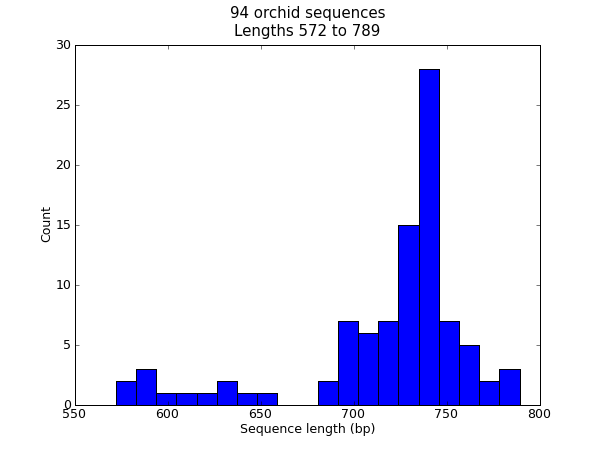
\includegraphics[width=0.8\textwidth]{images/hist_plot.png}
\caption{Histogram of orchid sequence lengths.}
\label{fig:seq-len-hist}
\end{figure}
\noindent That should pop up a new window containing the graph
shown in Figure~\ref{fig:seq-len-hist}.
\end{latexonly}
%
% The text now continues...
%
Notice that most of these orchid sequences are about $740$ bp long, and there could be
two distinct classes of sequence here with a subset of shorter sequences.

\emph{Tip:} Rather than using \verb|pylab.show()| to show the plot in a window,
you can also use \verb|pylab.savefig(...)| to save the figure to a file
(e.g. as a PNG or PDF).

\subsection{Plot of sequence GC\%}

Another easily calculated quantity of a nucleotide sequence is the GC\%.  You might
want to look at the GC\% of all the genes in a bacterial genome for example, and
investigate any outliers which could have been recently acquired by horizontal gene
transfer.  Again, for this example we'll reuse our orchid FASTA file
\href{https://raw.githubusercontent.com/biopython/biopython/master/Doc/examples/ls_orchid.fasta}{\tt ls\_orchid.fasta}.

First of all, we will use \verb|Bio.SeqIO| to parse the FASTA file and compile a list
of all the GC percentages.  Again, you could do this with a for loop, but I prefer this:

\begin{verbatim}
from Bio import SeqIO
from Bio.SeqUtils import GC

gc_values = sorted(GC(rec.seq) for rec in SeqIO.parse("ls_orchid.fasta", "fasta"))
\end{verbatim}

Having read in each sequence and calculated the GC\%, we then sorted them into ascending
order. Now we'll take this list of floating point values and plot them with matplotlib:

\begin{verbatim}
import pylab
pylab.plot(gc_values)
pylab.title("%i orchid sequences\nGC%% %0.1f to %0.1f" \
            % (len(gc_values),min(gc_values),max(gc_values)))
pylab.xlabel("Genes")
pylab.ylabel("GC%")
pylab.show()
\end{verbatim}

%
% Have an HTML version and a PDF version to display nicely...
%
\begin{htmlonly}
\noindent As in the previous example, that should pop up a new window containing a graph:

\imgsrc[width=600, height=450]{images/gc_plot.png}

\end{htmlonly}
%
% Now the PDF equivalent where we cannot always expect the figure
% to be positioned right next to the text, so we'll use a reference.
%
\begin{latexonly}
\begin{figure}[htbp]
\centering
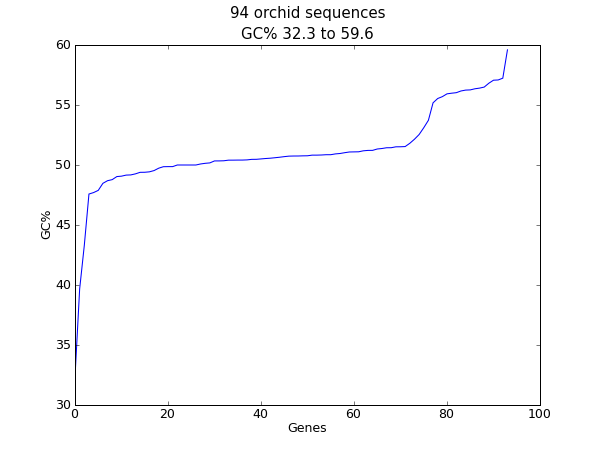
\includegraphics[width=0.8\textwidth]{images/gc_plot.png}
\caption{Histogram of orchid sequence lengths.}
\label{fig:seq-gc-plot}
\end{figure}
\noindent As in the previous example, that should pop up a new window with the graph shown in Figure~\ref{fig:seq-gc-plot}.
\end{latexonly}
%
% The text now continues...
%
If you tried this on the full set of genes from one organism, you'd probably get a much
smoother plot than this.

\subsection{Nucleotide dot plots}
A dot plot is a way of visually comparing two nucleotide sequences for similarity to
each other.  A sliding window is used to compare short sub-sequences to each other,
often with a mis-match threshold.  Here for simplicity we'll only look for perfect
matches (shown in black
\begin{latexonly}
in Figure~\ref{fig:nuc-dot-plot}).
\end{latexonly}
\begin{htmlonly}
in the plot below).
\end{htmlonly}

%
% Now the PDF equivalent where we cannot always expect the figure
% to be positioned right next to the text, so we'll use a reference.
%
\begin{latexonly}
\begin{figure}[htbp]
\centering
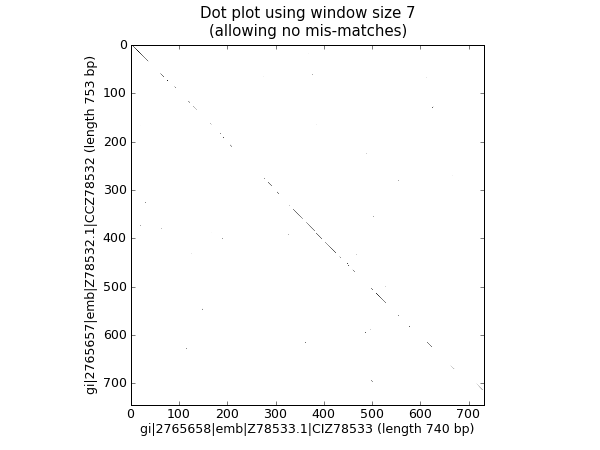
\includegraphics[width=0.8\textwidth]{images/dot_plot.png}
\caption{Nucleotide dot plot of two orchid sequence lengths (using pylab's imshow function).}
\label{fig:nuc-dot-plot}
\end{figure}
\end{latexonly}

To start off, we'll need two sequences.  For the sake of argument, we'll just take
the first two from our orchid FASTA file \href{https://raw.githubusercontent.com/biopython/biopython/master/Doc/examples/ls_orchid.fasta}{\tt ls\_orchid.fasta}:

\begin{verbatim}
from Bio import SeqIO
handle = open("ls_orchid.fasta")
record_iterator = SeqIO.parse(handle, "fasta")
rec_one = next(record_iterator)
rec_two = next(record_iterator)
handle.close()
\end{verbatim}

We're going to show two approaches.  Firstly, a simple naive implementation
which compares all the window sized sub-sequences to each other to compiles a
similarity matrix.  You could construct a matrix or array object, but here we
just use a list of lists of booleans created with a nested list
comprehension:

\begin{verbatim}
window = 7
seq_one = str(rec_one.seq).upper()
seq_two = str(rec_two.seq).upper()
data = [[(seq_one[i:i+window] <> seq_two[j:j+window]) \
        for j in range(len(seq_one)-window)] \
       for i in range(len(seq_two)-window)]
\end{verbatim}

Note that we have \emph{not} checked for reverse complement matches here.
Now we'll use the matplotlib's \verb|pylab.imshow()| function to display this
data, first requesting the gray color scheme so this is done in black and
white:

\begin{verbatim}
import pylab
pylab.gray()
pylab.imshow(data)
pylab.xlabel("%s (length %i bp)" % (rec_one.id, len(rec_one)))
pylab.ylabel("%s (length %i bp)" % (rec_two.id, len(rec_two)))
pylab.title("Dot plot using window size %i\n(allowing no mis-matches)" % window)
pylab.show()
\end{verbatim}
%pylab.savefig("dot_plot.png", dpi=75)
%pylab.savefig("dot_plot.pdf")

%
% Have a HTML version and a PDF version to display nicely...
%
\begin{htmlonly}
\noindent That should pop up a new window containing a graph like this:

\imgsrc[width=600, height=450]{images/dot_plot.png}

\end{htmlonly}
\begin{latexonly}
\noindent That should pop up a new window showing the graph in Figure~\ref{fig:nuc-dot-plot}.
\end{latexonly}
%
% The text now continues...
%
As you might have expected, these two sequences are very similar with a
partial line of window sized matches along the diagonal.  There are no off
diagonal matches which would be indicative of inversions or other interesting
events.

The above code works fine on small examples, but there are two problems
applying this to larger sequences, which we will address below.
First off all, this brute force approach to the all against all comparisons
is very slow.  Instead, we'll compile dictionaries mapping the window sized
sub-sequences to their locations, and then take the set intersection to find
those sub-sequences found in both sequences. This uses more memory, but is
\emph{much} faster.  Secondly, the \verb|pylab.imshow()| function is limited
in the size of matrix it can display.  As an alternative, we'll use the
\verb|pylab.scatter()| function.

We start by creating dictionaries mapping the window-sized sub-sequences to locations:
\begin{verbatim}
window = 7
dict_one = {}
dict_two = {}
for (seq, section_dict) in [(str(rec_one.seq).upper(), dict_one),
                            (str(rec_two.seq).upper(), dict_two)]:
    for i in range(len(seq)-window):
        section = seq[i:i+window]
        try:
            section_dict[section].append(i)
        except KeyError:
            section_dict[section] = [i]
#Now find any sub-sequences found in both sequences
#(Python 2.3 would require slightly different code here)
matches = set(dict_one).intersection(dict_two)
print("%i unique matches" % len(matches))
\end{verbatim}
\noindent In order to use the \verb|pylab.scatter()| we need separate lists for the $x$ and $y$ co-ordinates:
\begin{verbatim}
#Create lists of x and y co-ordinates for scatter plot
x = []
y = []
for section in matches:
    for i in dict_one[section]:
        for j in dict_two[section]:
            x.append(i)
            y.append(j)
\end{verbatim}
\noindent We are now ready to draw the revised dot plot as a scatter plot:
\begin{verbatim}
import pylab
pylab.cla() #clear any prior graph
pylab.gray()
pylab.scatter(x,y)
pylab.xlim(0, len(rec_one)-window)
pylab.ylim(0, len(rec_two)-window)
pylab.xlabel("%s (length %i bp)" % (rec_one.id, len(rec_one)))
pylab.ylabel("%s (length %i bp)" % (rec_two.id, len(rec_two)))
pylab.title("Dot plot using window size %i\n(allowing no mis-matches)" % window)
pylab.show()
\end{verbatim}
%pylab.savefig("dot_plot.png", dpi=75)
%pylab.savefig("dot_plot.pdf")
%
% Have a HTML version and a PDF version to display nicely...
%
\begin{htmlonly}
\noindent That should pop up a new window containing a graph like this:

\imgsrc[width=600, height=450]{images/dot_plot_scatter.png}

\end{htmlonly}
\begin{latexonly}
\noindent That should pop up a new window showing the graph in Figure~\ref{fig:nuc-dot-plot-scatter}.
\begin{figure}[htbp]
\centering
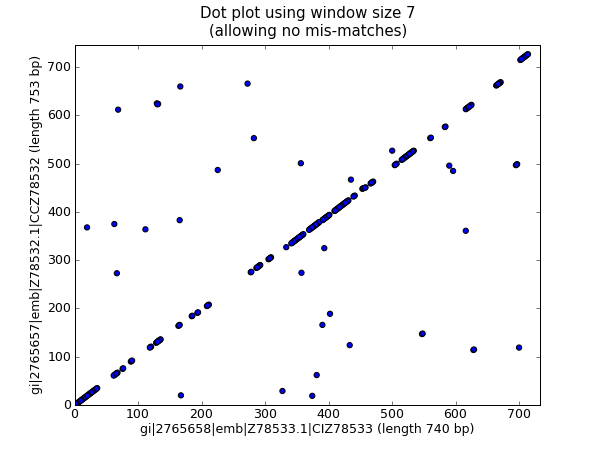
\includegraphics[width=0.8\textwidth]{images/dot_plot_scatter.png}
\caption{Nucleotide dot plot of two orchid sequence lengths (using pylab's scatter function).}
\label{fig:nuc-dot-plot-scatter}
\end{figure}\end{latexonly}
Personally I find this second plot much easier to read!
Again note that we have \emph{not} checked for reverse complement matches here
-- you could extend this example to do this, and perhaps plot the forward
matches in one color and the reverse matches in another.

\subsection{Plotting the quality scores of sequencing read data}

If you are working with second generation sequencing data, you may want to try plotting
the quality data. Here is an example using two FASTQ files containing paired end reads,
\texttt{SRR001666\_1.fastq} for the forward reads, and  \texttt{SRR001666\_2.fastq} for
the reverse reads. These were downloaded from the ENA sequence read archive FTP site
(\url{ftp://ftp.sra.ebi.ac.uk/vol1/fastq/SRR001/SRR001666/SRR001666_1.fastq.gz} and
\url{ftp://ftp.sra.ebi.ac.uk/vol1/fastq/SRR001/SRR001666/SRR001666_2.fastq.gz}), and
are from \textit{E. coli} -- see \url{http://www.ebi.ac.uk/ena/data/view/SRR001666}
for details.
%Originally from ftp://ftp.ncbi.nlm.nih.gov/sra/static/SRX000/SRX000430/

In the following code the \verb|pylab.subplot(...)| function is used in order to show
the forward and reverse qualities on two subplots, side by side. There is also a little
bit of code to only plot the first fifty reads.

\begin{verbatim}
import pylab
from Bio import SeqIO
for subfigure in [1,2]:
    filename = "SRR001666_%i.fastq" % subfigure
    pylab.subplot(1, 2, subfigure)
    for i,record in enumerate(SeqIO.parse(filename, "fastq")):
        if i >= 50 : break #trick!
        pylab.plot(record.letter_annotations["phred_quality"])
    pylab.ylim(0,45)
    pylab.ylabel("PHRED quality score")
    pylab.xlabel("Position")
pylab.savefig("SRR001666.png")
print("Done")
\end{verbatim}

You should note that we are using the \verb|Bio.SeqIO| format name \texttt{fastq}
here because the NCBI has saved these reads using the standard Sanger FASTQ format
with PHRED scores. However, as you might guess from the read lengths, this data was
from an Illumina Genome Analyzer and was probably originally in one of the two
Solexa/Illumina FASTQ variant file formats instead.

This example uses the \verb|pylab.savefig(...)| function instead of
\verb|pylab.show(...)|, but as mentioned before both are useful.
\begin{latexonly}
\begin{figure}[htbp]
\centering
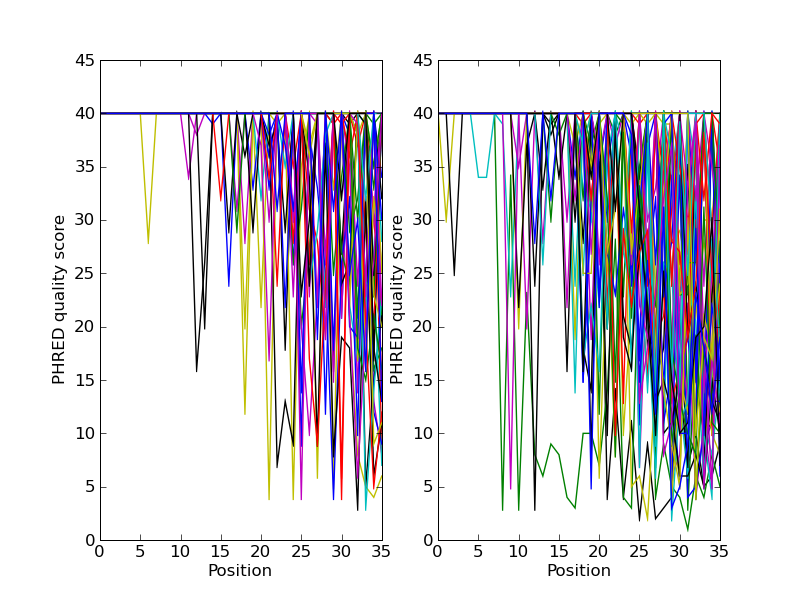
\includegraphics[width=0.8\textwidth]{images/SRR001666.png}
\caption{Quality plot for some paired end reads.}
\label{fig:paired-end-qual-plot}
\end{figure}
The result is shown in Figure~\ref{fig:paired-end-qual-plot}.
\end{latexonly}
\begin{htmlonly}
Here is the result:

%Blank lines here are important!
\imgsrc[width=600, height=600]{images/SRR001666.png}

\end{htmlonly}

\section{Dealing with alignments}

This section can been seen as a follow on to Chapter~\ref{chapter:Bio.AlignIO}.

\subsection{Calculating summary information}
\label{sec:summary_info}

Once you have an alignment, you are very likely going to want to find out information about it. Instead of trying to have all of the functions that can generate information about an alignment in the alignment object itself, we've tried to separate out the functionality into separate classes, which act on the alignment.

Getting ready to calculate summary information about an object is quick to do. Let's say we've got an alignment object called \verb|alignment|, for example read in using \verb|Bio.AlignIO.read(...)| as described in Chapter~\ref{chapter:Bio.AlignIO}. All we need to do to get an object that will calculate summary information is:

\begin{verbatim}
from Bio.Align import AlignInfo
summary_align = AlignInfo.SummaryInfo(alignment)
\end{verbatim}

The \verb|summary_align| object is very useful, and will do the following neat things for you:

\begin{enumerate}
  \item Calculate a quick consensus sequence -- see section~\ref{sec:consensus}
  \item Get a position specific score matrix for the alignment -- see section~\ref{sec:pssm}
  \item Calculate the information content for the alignment -- see section~\ref{sec:getting_info_content}
  \item Generate information on substitutions in the alignment -- section~\ref{sec:sub_matrix} details using this to generate a substitution matrix.
\end{enumerate}

\subsection{Calculating a quick consensus sequence}
\label{sec:consensus}

The \verb|SummaryInfo| object, described in section~\ref{sec:summary_info}, provides functionality to calculate a quick consensus of an alignment. Assuming we've got a \verb|SummaryInfo| object called \verb|summary_align| we can calculate a consensus by doing:

\begin{verbatim}
consensus = summary_align.dumb_consensus()
\end{verbatim}

As the name suggests, this is a really simple consensus calculator, and will just add up all of the residues at each point in the consensus, and if the most common value is higher than some threshold value will add the common residue to the consensus. If it doesn't reach the threshold, it adds an ambiguity character to the consensus. The returned consensus object is Seq object whose alphabet is inferred from the alphabets of the sequences making up the consensus. So doing a \verb|print consensus| would give:

\begin{verbatim}
consensus Seq('TATACATNAAAGNAGGGGGATGCGGATAAATGGAAAGGCGAAAGAAAGAAAAAAATGAAT
...', IUPACAmbiguousDNA())
\end{verbatim}

You can adjust how \verb|dumb_consensus| works by passing optional parameters:

\begin{description}
\item[the threshold] This is the threshold specifying how common a particular residue has to be at a position before it is added. The default is $0.7$ (meaning $70\%$).

\item[the ambiguous character] This is the ambiguity character to use. The default is 'N'.

\item[the consensus alphabet] This is the alphabet to use for the consensus sequence. If an alphabet is not specified than we will try to guess the alphabet based on the alphabets of the sequences in the alignment.
\end{description}

\subsection{Position Specific Score Matrices}
\label{sec:pssm}

Position specific score matrices (PSSMs) summarize the alignment information in a different way than a consensus, and may be useful for different tasks. Basically, a PSSM is a count matrix. For each column in the alignment, the number of each alphabet letters is counted and totaled. The totals are displayed relative to some representative sequence along the left axis. This sequence may be the consesus sequence, but can also be any sequence in the alignment. For instance for the alignment,

\begin{verbatim}
GTATC
AT--C
CTGTC
\end{verbatim}

\noindent the PSSM is:

\begin{verbatim}
      G A T C
    G 1 1 0 1
    T 0 0 3 0
    A 1 1 0 0
    T 0 0 2 0
    C 0 0 0 3
\end{verbatim}

Let's assume we've got an alignment object called \verb|c_align|. To get a PSSM with the consensus sequence along the side we first get a summary object and calculate the consensus sequence:

\begin{verbatim}
summary_align = AlignInfo.SummaryInfo(c_align)
consensus = summary_align.dumb_consensus()
\end{verbatim}

Now, we want to make the PSSM, but ignore any \verb|N| ambiguity residues when calculating this:

\begin{verbatim}
my_pssm = summary_align.pos_specific_score_matrix(consensus,
                                                  chars_to_ignore = ['N'])
\end{verbatim}

Two notes should be made about this:

\begin{enumerate}
  \item To maintain strictness with the alphabets, you can only include characters along the top of the PSSM that are in the alphabet of the alignment object. Gaps are not included along the top axis of the PSSM.

  \item The sequence passed to be displayed along the left side of the axis does not need to be the consensus. For instance, if you wanted to display the second sequence in  the alignment along this axis, you would need to do:

\begin{verbatim}
second_seq = alignment.get_seq_by_num(1)
my_pssm = summary_align.pos_specific_score_matrix(second_seq
                                                  chars_to_ignore = ['N'])
\end{verbatim}

\end{enumerate}

The command above returns a \verb|PSSM| object.
To print out the PSSM as shown above,
we simply need to do a \verb|print(my_pssm)|, which gives:

\begin{verbatim}
    A   C   G   T
T  0.0 0.0 0.0 7.0
A  7.0 0.0 0.0 0.0
T  0.0 0.0 0.0 7.0
A  7.0 0.0 0.0 0.0
C  0.0 7.0 0.0 0.0
A  7.0 0.0 0.0 0.0
T  0.0 0.0 0.0 7.0
T  1.0 0.0 0.0 6.0
...
\end{verbatim}

You can access any element of the PSSM by subscripting like \verb|your_pssm[sequence_number][residue_count_name]|. For instance, to get the counts for the 'A' residue in the second element of the above PSSM you would do:

\begin{verbatim}
>>> print(my_pssm[1]["A"])
7.0
\end{verbatim}

The structure of the PSSM class hopefully makes it easy both to access elements and to pretty print the matrix.

\subsection{Information Content}
\label{sec:getting_info_content}

A potentially useful measure of evolutionary conservation is the information content of a sequence.

A useful introduction to information theory targeted towards molecular biologists can be found at \url{http://www.lecb.ncifcrf.gov/~toms/paper/primer/}. For our purposes, we will be looking at the information content of a consesus sequence, or a portion of a consensus sequence. We calculate information content at a particular column in a multiple sequence alignment using the following formula:

\begin{displaymath}
IC_{j} = \sum_{i=1}^{N_{a}} P_{ij} \mathrm{log}\left(\frac{P_{ij}}{Q_{i}}\right)
\end{displaymath}

\noindent where:

\begin{itemize}
  \item $IC_{j}$ -- The information content for the $j$-th column in an alignment.
  \item $N_{a}$ -- The number of letters in the alphabet.
  \item $P_{ij}$ -- The frequency of a particular letter $i$ in the $j$-th column (i.~e.~if G occurred 3 out of 6 times in an aligment column, this would be 0.5)
  \item $Q_{i}$ --  The expected frequency of a letter $i$. This is an
  optional argument, usage of which is left at the user's
  discretion. By default, it is automatically assigned to $0.05 = 1/20$ for a
  protein alphabet, and $0.25 = 1/4$ for a nucleic acid alphabet. This is for
  geting the information content without any assumption of prior
  distributions. When assuming priors, or when using a non-standard
  alphabet, you should supply the values for $Q_{i}$.
\end{itemize}

Well, now that we have an idea what information content is being calculated in Biopython, let's look at how to get it for a particular region of the alignment.

First, we need to use our alignment to get an alignment summary object, which we'll assume is called \verb|summary_align| (see section~\ref{sec:summary_info}) for instructions on how to get this. Once we've got this object, calculating the information content for a region is as easy as:

\begin{verbatim}
info_content = summary_align.information_content(5, 30,
                                                 chars_to_ignore = ['N'])
\end{verbatim}

Wow, that was much easier then the formula above made it look! The variable \verb|info_content| now contains a float value specifying the information content over the specified region (from 5 to 30 of the alignment). We specifically ignore the ambiguity residue 'N' when calculating the information content, since this value is not included in our alphabet (so we shouldn't be interested in looking at it!).

As mentioned above, we can also calculate relative information content by supplying the expected frequencies:

\begin{verbatim}
expect_freq = {
    'A' : .3,
    'G' : .2,
    'T' : .3,
    'C' : .2}
\end{verbatim}

The expected should not be passed as a raw dictionary, but instead by passed as a \verb|SubsMat.FreqTable| object (see section~\ref{sec:freq_table} for more information about FreqTables). The FreqTable object provides a standard for associating the dictionary with an Alphabet, similar to how the Biopython Seq class works.

To create a FreqTable object, from the frequency dictionary you just need to do:

\begin{verbatim}
from Bio.Alphabet import IUPAC
from Bio.SubsMat import FreqTable

e_freq_table = FreqTable.FreqTable(expect_freq, FreqTable.FREQ,
                                   IUPAC.unambiguous_dna)
\end{verbatim}

Now that we've got that, calculating the relative information content for our region of the alignment is as simple as:

\begin{verbatim}
info_content = summary_align.information_content(5, 30,
                                                 e_freq_table = e_freq_table,
                                                 chars_to_ignore = ['N'])
\end{verbatim}

Now, \verb|info_content| will contain the relative information content over the region in relation to the expected frequencies.

The value return is calculated using base 2 as the logarithm base in the formula above. You can modify this by passing the parameter \verb|log_base| as the base you want:

\begin{verbatim}
info_content = summary_align.information_content(5, 30, log_base = 10,
                                                 chars_to_ignore = ['N'])
\end{verbatim}

Well, now you are ready to calculate information content. If you want to try applying this to some real life problems, it would probably be best to dig into the literature on information content to get an idea of how it is used. Hopefully your digging won't reveal any mistakes made in coding this function!

\section{Substitution Matrices}
\label{sec:sub_matrix}

Substitution matrices are an extremely important part of everyday bioinformatics work. They provide the scoring terms for classifying how likely two different residues are to substitute for each other. This is essential in doing sequence comparisons. The book ``Biological Sequence Analysis'' by Durbin et al. provides a really nice introduction to Substitution Matrices and their uses. Some famous substitution matrices are the PAM and BLOSUM series of matrices.

Biopython provides a ton of common substitution matrices, and also provides functionality for creating your own substitution matrices.

\subsection{Using common substitution matrices}

\subsection{Creating your own substitution matrix from an alignment}
\label{sec:subs_mat_ex}

A very cool thing that you can do easily with the substitution matrix
classes is to create your own substitution matrix from an
alignment. In practice, this is normally done with protein
alignments. In this example, we'll first get a Biopython alignment
object and then get a summary object to calculate info about the
alignment. The file containing \href{examples/protein.aln}{protein.aln}
(also available online
\href{https://raw.githubusercontent.com/biopython/biopython/master/Doc/examples/protein.aln}{here})
contains the Clustalw alignment output.

%doctest examples
\begin{verbatim}
>>> from Bio import AlignIO
>>> from Bio import Alphabet
>>> from Bio.Alphabet import IUPAC
>>> from Bio.Align import AlignInfo
>>> filename = "protein.aln"
>>> alpha = Alphabet.Gapped(IUPAC.protein)
>>> c_align = AlignIO.read(filename, "clustal", alphabet=alpha)
>>> summary_align = AlignInfo.SummaryInfo(c_align)
\end{verbatim}

Sections~\ref{sec:align_clustal} and~\ref{sec:summary_info} contain
more information on doing this.

Now that we've got our \verb|summary_align| object, we want to use it
to find out the number of times different residues substitute for each
other. To make the example more readable, we'll focus on only amino
acids with polar charged side chains. Luckily, this can be done easily
when generating a replacement dictionary, by passing in all of the
characters that should be ignored. Thus we'll create a dictionary of
replacements for only charged polar amino acids using:

%cont-doctest
\begin{verbatim}
>>> replace_info = summary_align.replacement_dictionary(["G", "A", "V", "L", "I",
...                                                      "M", "P", "F", "W", "S",
...                                                      "T", "N", "Q", "Y", "C"])
\end{verbatim}

This information about amino acid replacements is represented as a
python dictionary which will look something like (the order can vary):

\begin{verbatim}
{('R', 'R'): 2079.0, ('R', 'H'): 17.0, ('R', 'K'): 103.0, ('R', 'E'): 2.0,
('R', 'D'): 2.0, ('H', 'R'): 0, ('D', 'H'): 15.0, ('K', 'K'): 3218.0,
('K', 'H'): 24.0, ('H', 'K'): 8.0, ('E', 'H'): 15.0, ('H', 'H'): 1235.0,
('H', 'E'): 18.0, ('H', 'D'): 0, ('K', 'D'): 0, ('K', 'E'): 9.0,
('D', 'R'): 48.0, ('E', 'R'): 2.0, ('D', 'K'): 1.0, ('E', 'K'): 45.0,
('K', 'R'): 130.0, ('E', 'D'): 241.0, ('E', 'E'): 3305.0,
('D', 'E'): 270.0, ('D', 'D'): 2360.0}
\end{verbatim}

This information gives us our accepted number of replacements, or how
often we expect different things to substitute for each other. It
turns out, amazingly enough, that this is all of the information we
need to go ahead and create a substitution matrix. First, we use the
replacement dictionary information to create an Accepted Replacement
Matrix (ARM):

%cont-doctest
\begin{verbatim}
>>> from Bio import SubsMat
>>> my_arm = SubsMat.SeqMat(replace_info)
\end{verbatim}

With this accepted replacement matrix, we can go right ahead and
create our log odds matrix (i.~e.~a standard type Substitution Matrix):

%cont-doctest
\begin{verbatim}
>>> my_lom = SubsMat.make_log_odds_matrix(my_arm)
\end{verbatim}

The log odds matrix you create is customizable with the following
optional arguments:

\begin{itemize}
  \item \verb|exp_freq_table| -- You can pass a table of expected
  frequencies for each alphabet. If supplied, this will be used
  instead of the passed accepted replacement matrix when calculate
  expected replacments.

  \item \verb|logbase| - The base of the logarithm taken to create the
  log odd matrix. Defaults to base 10.

  \item \verb|factor| - The factor to multiply each matrix entry
  by. This defaults to 10, which normally makes the matrix numbers
  easy to work with.

  \item \verb|round_digit| - The digit to round to in the matrix. This
  defaults to 0 (i.~e.~no digits).

\end{itemize}

Once you've got your log odds matrix, you can display it prettily
using the function \verb|print_mat|. Doing this on our created matrix
gives:

%cont-doctest
\begin{verbatim}
>>> my_lom.print_mat()
D   2
E  -1   1
H  -5  -4   3
K -10  -5  -4   1
R  -4  -8  -4  -2   2
   D   E   H   K   R
\end{verbatim}

Very nice. Now we've got our very own substitution matrix to play with!

\section{BioSQL -- storing sequences in a relational database}
\label{sec:BioSQL}
\href{http://www.biosql.org/}{BioSQL} is a joint effort between the
\href{http://open-bio.org/}{OBF} projects (BioPerl, BioJava etc) to support a
shared database schema for storing sequence data. In theory, you could load a
GenBank file into the database with BioPerl, then using Biopython extract this
from the database as a record object with features - and get more or less the same
thing as if you had loaded the GenBank file directly as a SeqRecord using
\verb|Bio.SeqIO| (Chapter~\ref{chapter:Bio.SeqIO}).

Biopython's BioSQL module is currently documented at
\url{http://biopython.org/wiki/BioSQL} which is part of our wiki pages.

